\documentclass[12pt,a4paper]{article}
\usepackage[utf8]{inputenc}
\usepackage{geometry}
\usepackage{graphicx}
\usepackage{hyperref}
\usepackage{array}
\usepackage{booktabs}
\usepackage{enumitem}
\usepackage{float}
\usepackage{titlesec}
\usepackage{fancyhdr}
\usepackage{xcolor}
\usepackage{ragged2e}

\geometry{top=0.8in,bottom=0.9in,left=0.5in,right=0.5in}

\title{\textbf{Agentic Terminal Bot for Environment Setup \& Debugging} \\ \large Project Report}
\author{
  \textbf{MUKUL GHARE} --- 25345960 \\
  \textbf{YIFAN LI} --- 25333983 \\
  \textbf{DAVID KONOVALOVS} --- 21364153 \\
  \textbf{SAI EESHWAR DIVAAKAR} --- 25338829 \\
  \textbf{SNEHA METO} --- 25337472 \\
  \\
  \textbf{Group: Cagney \& Lacey}
}
\date{\today}

\pagestyle{fancy}
\fancyhf{}
\rhead{\thepage}
\lhead{Shellock Project Outline}

\begin{document}
\justifying 

\maketitle


\tableofcontents

% ============================================================
\section{Introduction}
% ============================================================

\subsection{Motivation}
Modern development work is increasingly dominated by ``environment work'': creating isolated runtimes, installing
dependencies, aligning toolchains across operating systems, and repeatedly diagnosing common failures such as missing
modules or version mismatches. While automation scripts can reduce manual effort, they tend to be brittle and project-
specific. On the other hand, AI-based assistants can be powerful, but often behave like black boxes and may take
unsafe actions if not carefully constrained.\cite{amershi2019,shneiderman2020}
Shellock is motivated by the need for an assistant that is both \emph{helpful} and \emph{trustworthy}: it should adapt
to user preferences over time, remain fully inspectable and user-controlled, and work across heterogeneous terminal
environments (including offline or low-connectivity settings).\cite{amershi2019,shneiderman2020}

\subsection{Project Goal}
The goal of this project is to build \textbf{Shellock}, an \emph{adaptive terminal environment orchestrator} and
\emph{human-gated Large Action Model (LAM)} for developer environment setup and error diagnosis. Given a natural-
language intent (e.g., ``python 3.11 fastapi project with black'') or a concrete failure (e.g.,
\texttt{ModuleNotFoundError}), Shellock produces a structured plan, proposes a validated sequence of terminal actions,
and executes them \emph{only after explicit user approval}.\cite{amershi2019,shneiderman2020}
To make this practical and safe, Shellock targets: (1) adaptability via deterministic preference learning, (2)
scrutability via transparent specs and audit trails, and (3) universal compatibility via modular design with offline-
first operation (local LLM) and a non-LLM template fallback.

\subsection{Methodology}
We adopt an iterative, architecture-first methodology aligned with the adaptive loop:
\begin{quote}
Perceive $\rightarrow$ Plan $\rightarrow$ Human Approve $\rightarrow$ Execute $\rightarrow$ Observe $\rightarrow$
Adapt.
\end{quote}
System design choices prioritize safety and reliability: the LLM is constrained to text-to-structured-spec
transformation rather than direct command execution; all commands are checked against module allowlists and blocked-
pattern rules; and the system maintains an auditable history of actions and outcomes.\cite{amershi2019,shneiderman2020} Implementation is organized
around a small core (context detection, spec schemas, dispatcher, registry, UI) plus pluggable ecosystem modules
(Python/Node) that generate environment and diagnosis actions. Correctness is supported through automated tests
covering schemas, dispatch/validation behavior, module logic, and CLI workflows.

\subsection{Report Outline}
The remainder of this report is organized as follows. We first describe the problem setting and the design principles
that guide Shellock (adaptability, scrutability, and compatibility). Next, we present the system architecture and key
components (CLI/UI, context detection, module loading, dispatcher and safety checks, registry and audit trail, and
LLM/fallback pipeline). We then detail the implementation of the built-in Python and Node modules and the error-
diagnosis escalation strategy. Finally, we evaluate the system through test coverage and representative end-to-end
scenarios, discuss limitations and future improvements, and conclude with a summary of contributions.
% % ============================================================
% \section{Introduction}
% % ============================================================

% \subsection{Motivation}

% \subsection{Project Goal}

% \subsection{Methodology}

% \subsection{Report Outline}

% ============================================================
\section{User Modelling}
% ============================================================

\subsection{Modelling Techniques}

Shellock uses an \emph{explicit, deterministic} user model designed for scrutability and privacy. Instead of implicit
profiling or black-box learning, it records only the minimum information required to adapt: (1) frequency counts of
user-confirmed tool choices (preferences), and (2) a small set of user-controlled thresholds and exclusions that gate
when adaptation is allowed. This technique is intentionally simple and inspectable: the model is stored locally as a
human-readable JSON file and can be viewed at any time via the CLI.\cite{kobsa2001,brusilovsky2007,amershi2019}

Figure~\ref{fig:use-case} summarises the main user interactions that provide signals for adaptation.\cite{omguml} Importantly, the
``Human Approve'' step remains a first-class use case: Shellock may \emph{suggest} actions based on past choices, but it
does not execute any command without user confirmation.

\begin{figure}[H]
  \centering
  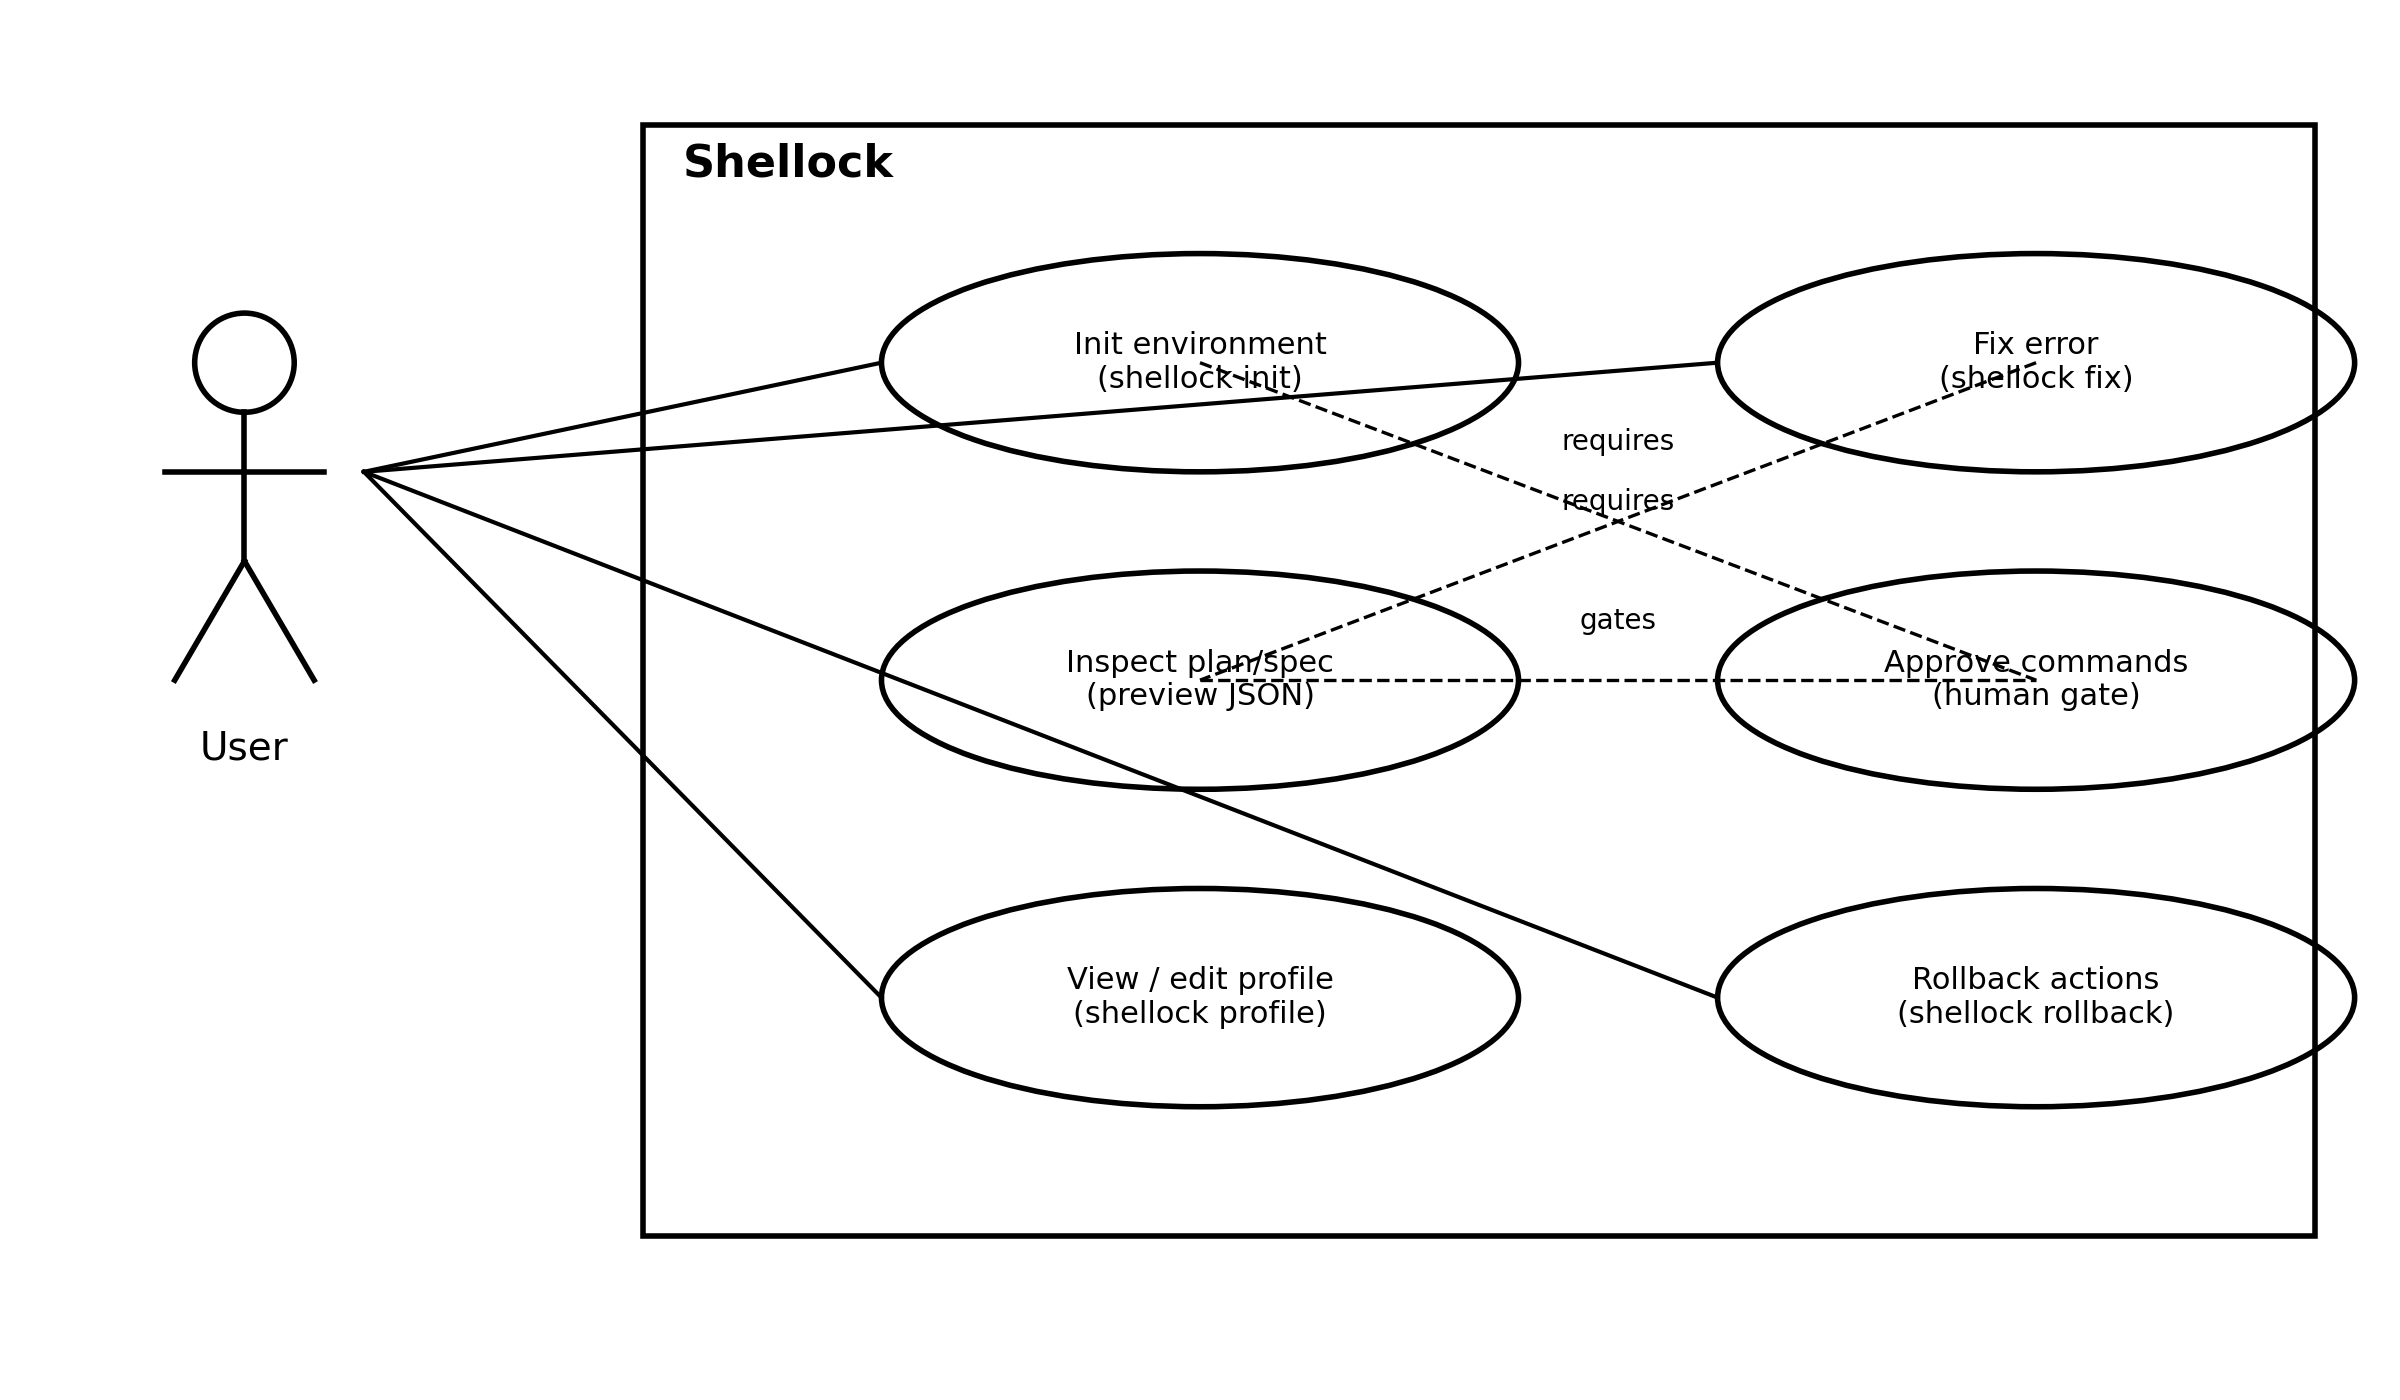
\includegraphics[width=0.95\linewidth]{images/use_case.png}
  \caption{Use case diagram for user-modelling and human-gated execution in Shellock.}
  \label{fig:use-case}
\end{figure}

\subsection{The User Model (\texttt{UserProfile})}

The core user model is \texttt{UserProfile}, implemented as a \texttt{Pydantic} schema and persisted in
\texttt{\textasciitilde/.shellock/profile.json}.\cite{pydantic,kobsa2001} It captures both \emph{preferences} (what the user repeatedly selects)
and \emph{context} (auto-detected system capabilities) in a single, auditable structure. Figure~\ref{fig:user-model}
shows the main fields and how preference learning feeds into adaptive suggestions.

\begin{figure}[H]
  \centering
  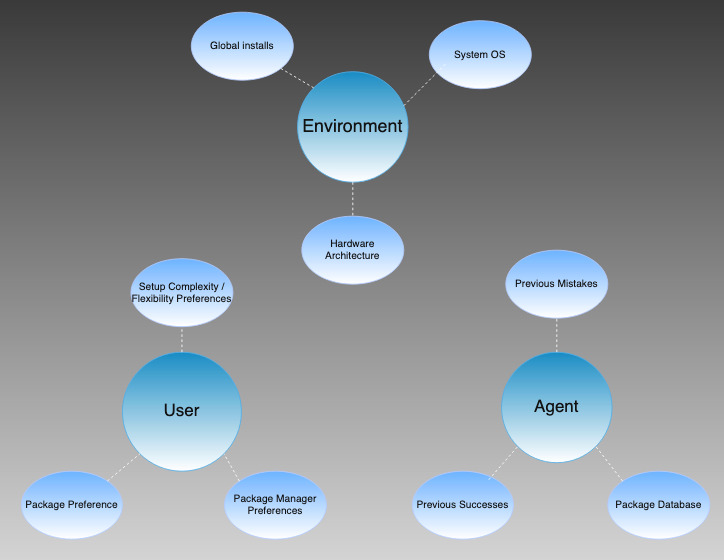
\includegraphics[width=0.92\linewidth]{images/user_model.png}
  \caption{\texttt{UserProfile} overview: deterministic preferences and the control parameters that gate adaptation.}
  \label{fig:user-model}
\end{figure}

At a high level, \texttt{UserProfile} contains:
\begin{itemize}
  \item \texttt{preferences: dict[str, dict[str, int]]} --- category $\rightarrow$ tool usage counters (e.g.,
  \texttt{tools}, \texttt{formatter}).
  \item \texttt{suggestion\_threshold: int} --- minimum count before a tool becomes eligible for auto-suggestion.
  \item \texttt{rejected\_suggestions: list[str]} --- explicit user opt-out list; tools here are never suggested.
  \item \texttt{system: SystemInfo} --- auto-detected OS/shell/LLM tier and hardware summary used for context-aware
  behaviour.
\end{itemize}

\subsubsection{Preference Tracking}

Preference tracking is implemented as \emph{monotonic counters} recorded only after the user has explicitly approved a
plan. After a successful run, Shellock iterates over the tools included in the environment specification and increments
the corresponding counters (via \texttt{record\_choice(category, tool)}). The data is stored as a simple nested map:
\begin{quote}
\texttt{\{tools: \{black: 5, ruff: 1\}\}}
\end{quote}
This representation is intentionally transparent: it supports easy inspection, manual editing, and deterministic
behaviour across runs. No telemetry or remote synchronisation is required; the model is purely local.

\subsubsection{Suggestion Threshold and Adaptive Axis}

To avoid premature or unwanted automation, Shellock gates adaptation with a \texttt{suggestion\_threshold} (default
\texttt{3}). A tool is eligible for suggestion only if its count is greater than or equal to the threshold, it is not
already present in the current spec (exclusion list), and it has not been explicitly rejected by the user.

This mechanism forms \textbf{Adaptive Axis 1 (User Preferences)} in the adaptive engine. During spec construction, the
system queries \texttt{UserProfile.get\_suggestions()} and, for each eligible tool, announces the adaptation in the UI
before adding it to the proposed package list. The result is an adaptive behaviour that is both effective (reducing
repeated configuration work) and scrutable (the user can see \emph{why} a tool was suggested and can still veto the
final command execution).

\subsection{System Context Detection}

\subsubsection{Hardware Detection (CPU, GPU, VRAM)}

\subsubsection{LLM Tier Detection}

% % ============================================================
% \section{System Architecture and Technology Stack}
% % ============================================================

% \subsection{Architectural Overview}

% \subsubsection{CLI Layer (\texttt{Typer})}

% \subsubsection{Core Layer (Dispatcher, Registry, LLM Client)}

% \subsubsection{Module Layer (Python, Node)}

% \subsection{Implemented Technology}

% \subsubsection{Pydantic Schemas}

% \subsubsection{LLM Integration (\texttt{Ollama}, \texttt{Gemini})}

% \subsubsection{Command Safety and Allowlist}

% ============================================================
\section{System Architecture and Technology Stack}
% ============================================================

\subsection{Architectural Overview}

Shellock is a \emph{human-gated} terminal assistant that turns natural-language intent into a
structured environment specification (EnvSpec), validates it, and only then executes the
corresponding shell commands. The architecture follows a layered design, comprising a Typer-based CLI
front-end, a core orchestration layer, and a pluggable module layer for ecosystem-specific logic.\cite{parnas1972} 
 
As illustrated in Figure~\ref{fig:concept-architecture}, the conceptual design prioritizes a 
separation between presentation, logic, and infrastructure, featuring an explicit user approval 
gate to ensure safety. The implemented version of this architecture is detailed in 
Figure~\ref{fig:impl-architecture}, which showcases the interaction between core services 
and ecosystem modules.

\begin{figure}[H]
  \centering
  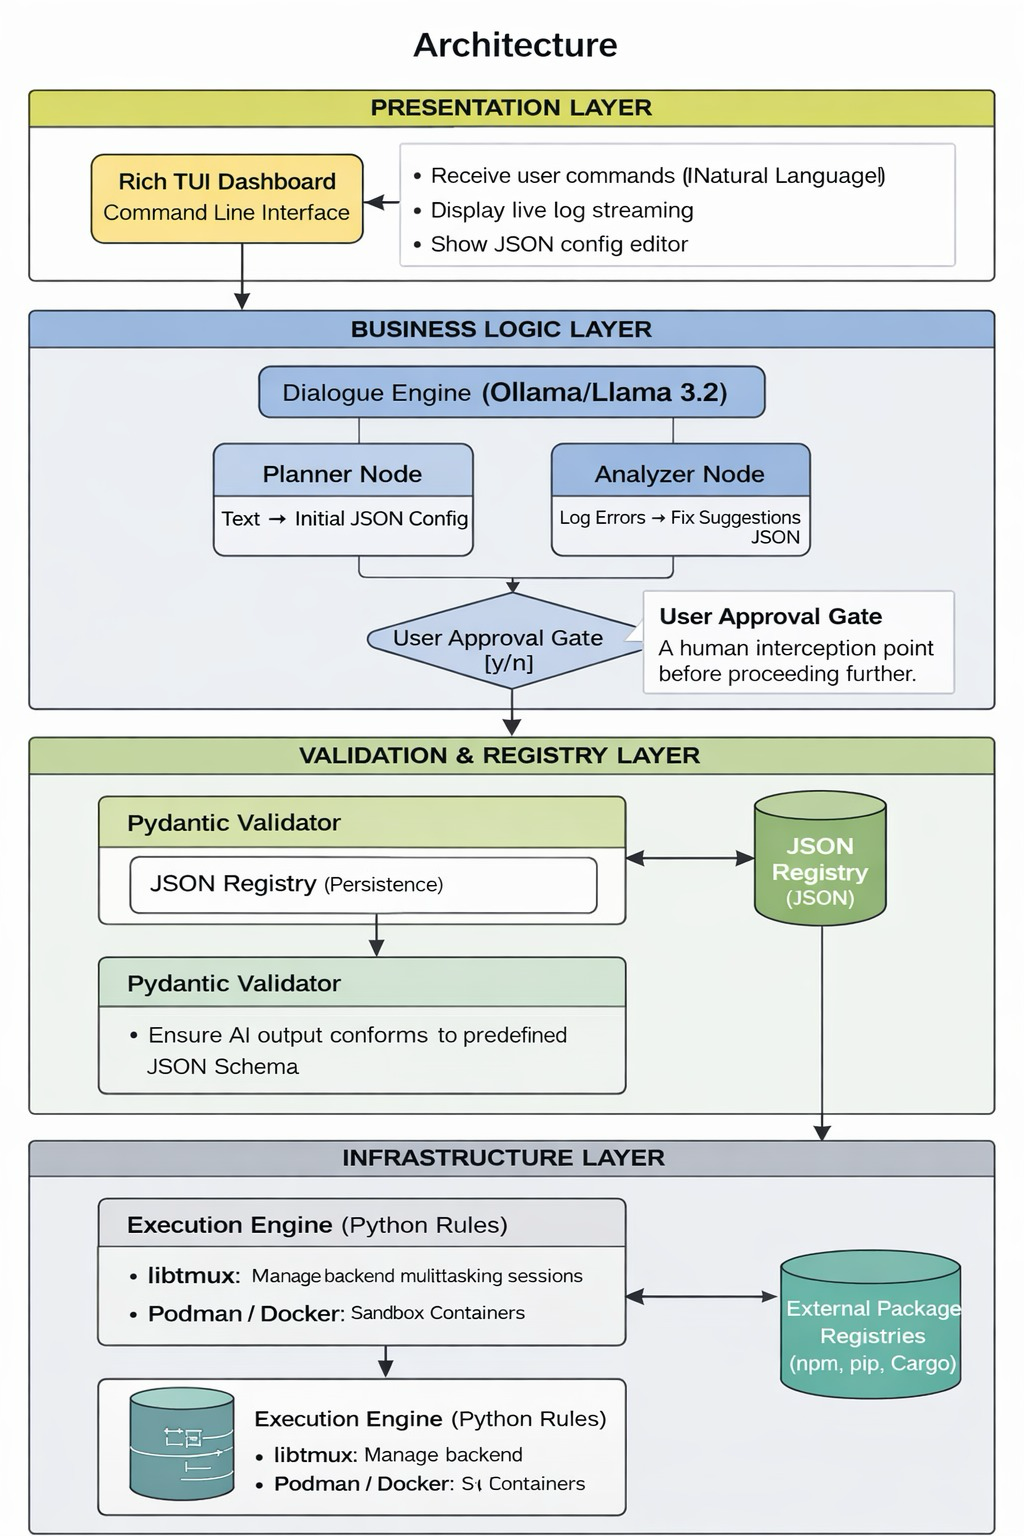
\includegraphics[width=0.9\linewidth]{images/texhStack.png}
  \caption{Conceptual Architecture}
  \label{fig:concept-architecture}
\end{figure}

\begin{figure}[H]
  \centering
  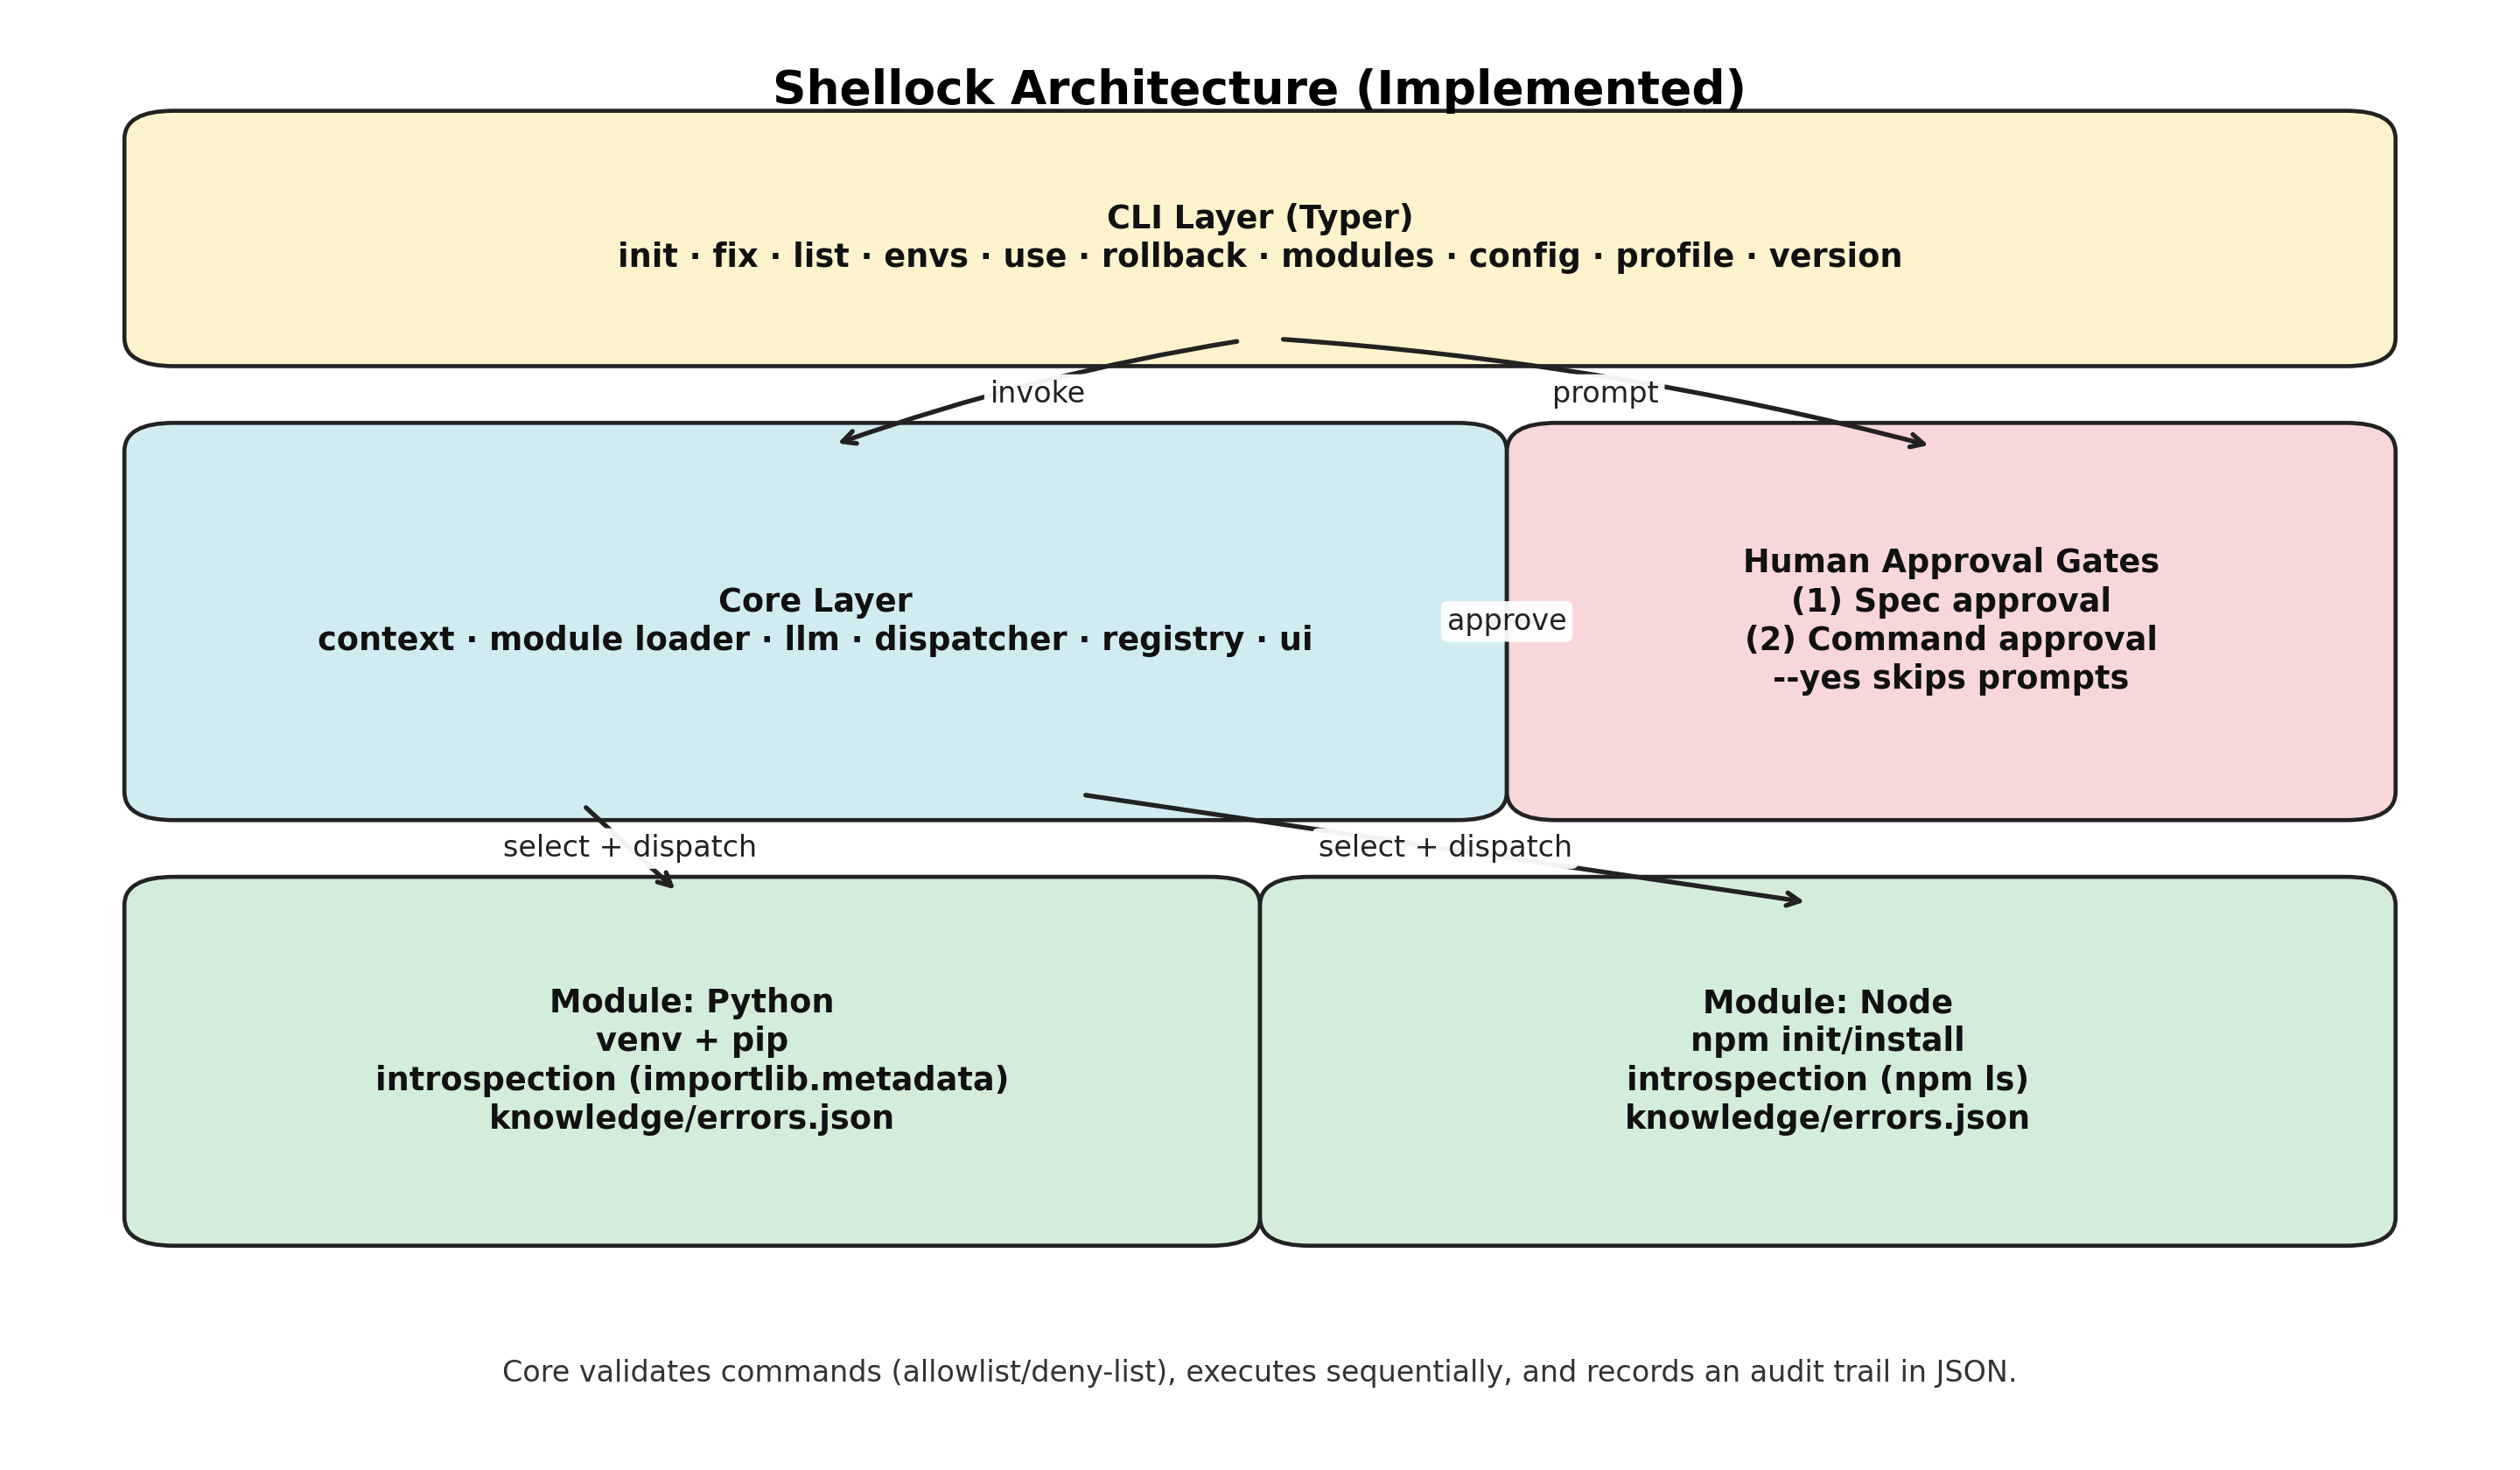
\includegraphics[width=\linewidth]{images/shellock_architecture.png}
  \caption{Implemented Architecture}
  \label{fig:impl-architecture}
\end{figure}

\subsubsection{CLI Layer (\texttt{Typer})}

The CLI is implemented using \texttt{Typer} and exposed as the \texttt{shellock} executable via the
Python packaging entry point. The CLI aggregates all user-facing commands, including environment 
creation and diagnosis workflows such as \texttt{init}, \texttt{fix}, and \texttt{rollback}. 
On first invocation, a one-time onboarding wizard populates a local user profile based on 
detected system capabilities.\cite{typer}

\subsubsection{Core Layer (Dispatcher, Registry, LLM Client)}

The core layer orchestrates the end-to-end adaptive loop:

\begin{itemize}
  \item \textbf{Context detection:} \texttt{context.py} deterministically detects OS, shell, and 
  available package managers to enrich prompts and spec previews.
  \item \textbf{LLM client:} \texttt{llm.py} handles structured output generation. It is strictly 
  responsible for text-to-JSON conversion and does not execute commands.
  \item \textbf{Dispatcher:} \texttt{dispatcher.py} serves as the single execution point, running 
  validated commands and capturing outputs for auditing.
  \item \textbf{Registry:} \texttt{registry.py} manages persistence for global configs and 
  per-project history, enabling error fingerprinting and rollbacks.
\end{itemize}

\subsubsection{Module Layer (Python, Node)}

Shellock uses a module interface to isolate ecosystem-specific logic. Each module handles spec 
generation, command dispatch, and introspection-first diagnosis using native tools (e.g., \texttt{npm} or \texttt{pip}).

\subsection{Implemented Technology}

\subsubsection{Pydantic Schemas}

All key data structures are defined as \texttt{Pydantic} models. These schemas act as the system's 
source of truth, forbidding extra fields to ensure that LLM outputs are safely consumed without 
unexpected side effects.\cite{pydantic}

\subsubsection{LLM Integration (\texttt{Ollama}, \texttt{Gemini})}

Shellock supports a tiered LLM strategy, ranging from a \textbf{Local tier} using \texttt{Ollama} 
for privacy, to a \textbf{Cloud tier} via \texttt{Gemini 2.0 Flash}. A template fallback ensures 
functionality even when no LLM is reachable.\cite{ollama,gemini}

\subsubsection{Command Safety and Allowlist}

Safety is enforced through a multi-layered pipeline as shown in Figure~\ref{fig:cmd-safety}. 
This process includes module-based allowlists, regex-driven blocked patterns, and mandatory 
human approval gates to verify the impact of proposed commands.

\begin{figure}[H]
  \centering
  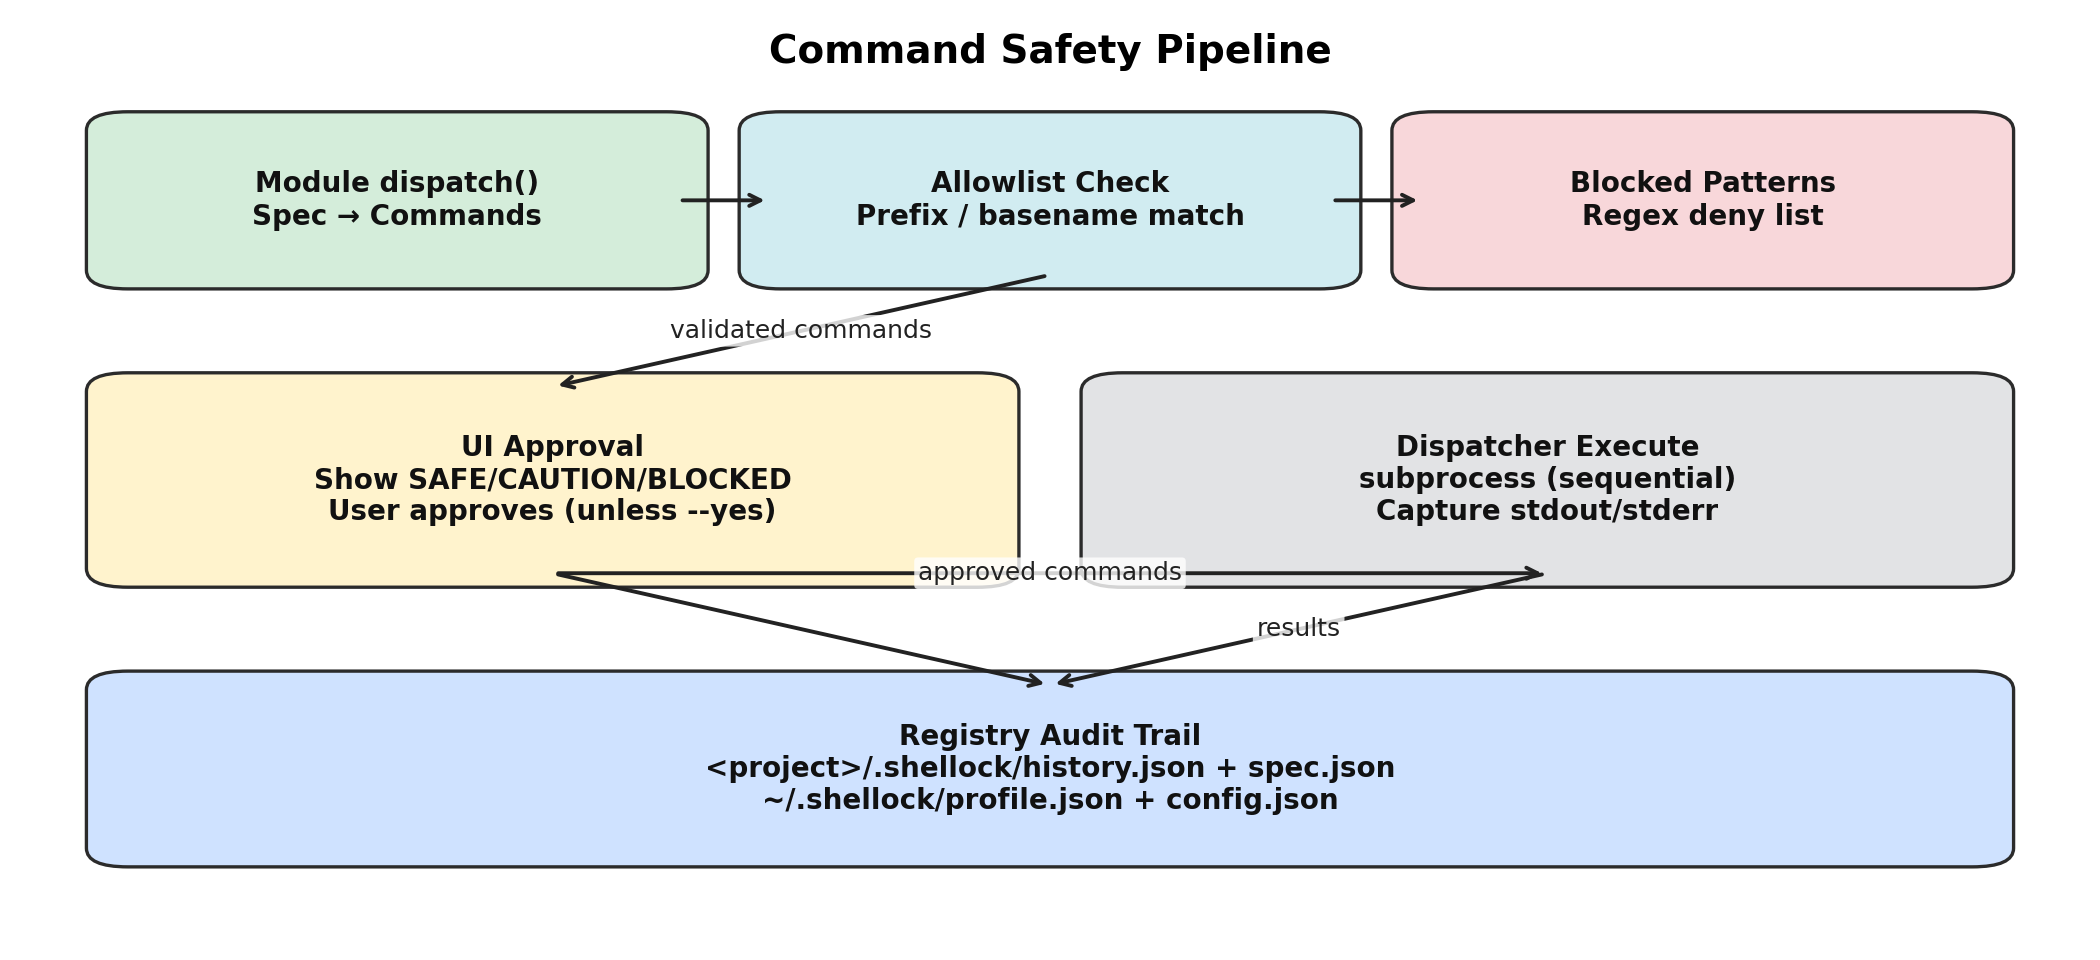
\includegraphics[width=\linewidth]{images/shellock_safety_pipeline.png}
  \caption{Safety Pipeline}
  \label{fig:cmd-safety}
\end{figure}

The implementation process was further supported by a robust engineering toolchain, 
including source control and project tracking systems, as depicted in Figure~\ref{fig:management}.

\begin{figure}[H]
  \centering
  
\includegraphics[width=0.9\linewidth]{images/management.png}
  \caption{Engineering Tooling}
  \label{fig:management}
\end{figure}

% ============================================================
\section{Implementation}
% ============================================================

\subsection{LLM-Driven Spec Generation}

\subsubsection{Tier Fallback (Cloud $\to$ Local $\to$ Template)}

\subsubsection{Template Mode and Keyword Inference}

\subsection{Environment Initialisation (\texttt{shellock init})}

\subsubsection{Module Detection and AST Import Scanning}

\subsubsection{Knowledge Enrichment and Package Correction}

\subsubsection{Web Search Integration (\texttt{Serper})}

\subsubsection{Approval and Edit Flow}

\subsection{Error Diagnosis and Self-Repair (\texttt{shellock fix})}

\subsubsection{Fingerprinting and Cascading Error Detection}

\subsubsection{Layered Diagnosis (Regex $\to$ Heuristic $\to$ LLM)}

\subsubsection{Fix Recording and Reuse}

\subsection{Command Dispatch and Safety}

\subsubsection{Allowlist Validation}

\subsubsection{Shell Metacharacter Blocking}

\subsubsection{Rollback Support}

\subsection{User Interface and Terminal Output}

\subsubsection{Rich vs.\ Plain Mode}

\subsubsection{Approval Screen and Spec Editor}

\subsection{Persistence and Audit Trail}

\subsubsection{Registry and Action History}

\subsubsection{Export Formats (\texttt{JSON}, \texttt{requirements.txt}, 
    \texttt{Dockerfile}, \texttt{devcontainer})}

% ============================================================
\section{Evaluation}
% ============================================================

\subsection{Adaptivity --- Does It Learn?}

\subsection{Accuracy of Package Inference (LLM vs.\ Template)}

\subsection{Fix Success Rate}

\subsection{Performance (Detection Latency)}

% ============================================================
\section{Conclusion and Future Work}

jkhsdkuhoidjaslkxc
% ============================================================

% ============================================================
\begin{thebibliography}{99}

\bibitem{amershi2019}
Saleema Amershi, Dan Weld, Mihaela Vorvoreanu, Adam Fourney, Besmira Nushi, Penny Collisson, Jina Suh, Shamsi Iqbal,
Paul N. Bennett, Kori Inkpen, et al.
\newblock Guidelines for Human--AI Interaction.
\newblock In \emph{Proceedings of the 2019 CHI Conference on Human Factors in Computing Systems (CHI '19)}, ACM, 2019.

\bibitem{shneiderman2020}
Ben Shneiderman.
\newblock Human-Centered Artificial Intelligence: Reliable, Safe \& Trustworthy.
\newblock \emph{International Journal of Human--Computer Interaction}, 36(6):495--504, 2020.

\bibitem{kobsa2001}
Alfred Kobsa.
\newblock Generic User Modeling Systems.
\newblock \emph{User Modeling and User-Adapted Interaction}, 11:49--63, 2001.

\bibitem{brusilovsky2007}
Peter Brusilovsky and Eva Mill{\'a}n.
\newblock User Models for Adaptive Hypermedia and Adaptive Educational Systems.
\newblock In Peter Brusilovsky, Alfred Kobsa, and Wolfgang Nejdl (eds.), \emph{The Adaptive Web}, Lecture Notes in
Computer Science 4321, Springer, 2007.

\bibitem{parnas1972}
David L. Parnas.
\newblock On the Criteria To Be Used in Decomposing Systems into Modules.
\newblock \emph{Communications of the ACM}, 15(12):1053--1058, 1972.

\bibitem{omguml}
Object Management Group.
\newblock Unified Modeling Language (UML), Version 2.5.1.
\newblock 2017. \url{https://www.omg.org/spec/UML/2.5.1}. Accessed 2026-04-12.

\bibitem{typer}
Sebasti{\'a}n Ram{\'i}rez.
\newblock Typer: modern CLI framework for Python.
\newblock \url{https://typer.tiangolo.com/}. Accessed 2026-04-12.

\bibitem{pydantic}
Samuel Colvin and contributors.
\newblock Pydantic: data validation using Python type hints.
\newblock \url{https://docs.pydantic.dev/}. Accessed 2026-04-12.

\bibitem{ollama}
Ollama contributors.
\newblock Ollama documentation.
\newblock \url{https://ollama.com/}. Accessed 2026-04-12.

\bibitem{gemini}
Google.
\newblock Gemini API documentation.
\newblock \url{https://ai.google.dev/gemini-api}. Accessed 2026-04-12.

\end{thebibliography}
% ============================================================

\end{document}
